
\documentclass[11pt,a4paper]{article}
\usepackage[T1]{fontenc}
\usepackage[utf8]{inputenc}
\usepackage[portuguese]{babel}
\usepackage{amsmath,amssymb,graphicx,booktabs,geometry,caption,float,indentfirst}
\usepackage[colorlinks=true,linkcolor=black,citecolor=black,urlcolor=blue]{hyperref}
\geometry{margin=2.4cm}
\captionsetup{font=small,labelfont=bf}
\setlength{\parskip}{2pt}

\title{\textbf{Medida da Velocidade da Luz pelo Método da Modulação de Fase}\\[2pt]
\large Experimento 5 --- Física Experimental (kit PHYWE 1329)\\[4pt]
\normalsize Simulação computacional do aparato e tratamento estatístico dos dados}
\author{Universidade Federal do Acre --- Centro de Ciências Biológicas e da Natureza}
\date{\today}

\begin{document}
\maketitle

\begin{abstract}
\noindent
Mediu-se a velocidade da luz no ar pelo método da comparação de fase entre um feixe
de luz modulado em intensidade a $\nu = 50{,}1$~MHz e o sinal de referência do
emissor, usando a abertura da figura de Lissajous no osciloscópio como fasímetro.
A partir de cinco medidas obteve-se
$c = (2{,}9649 \pm 0{,}0298)\times 10^{8}$~m/s, compatível com o valor aceito
dentro de 1{,}1 desvios-padrão (discrepância de 1{,}10\%). Um ajuste linear
de $\phi(\Delta x)$ forneceu $c = (2{,}9964 \pm 0{,}0847)\times 10^{8}$~m/s e o
método complementar do deslocamento de meia onda, $c = (2{,}9975 \pm 0{,}0066)\times
10^{8}$~m/s. Para os meios transparentes obtiveram-se
$n_{\text{água}} = 1{,}3391 \pm 0{,}0033$ e
$n_{\text{resina}} = 1{,}5104 \pm 0{,}0112$, correspondendo a
$c_{\text{água}} = (2{,}2140 \pm 0{,}0229)\times10^{8}$~m/s e
$c_{\text{resina}} = (1{,}9630 \pm 0{,}0245)\times10^{8}$~m/s. Discute-se por que
o método mede a velocidade \emph{de grupo} e não a de fase.
\end{abstract}

\section{Objetivos}
Medir a velocidade da luz no ar e, em seguida, em dois meios transparentes
(água destilada e resina sintética), determinando os respectivos índices de
refração; aplicar a regra de propagação de erros para grandezas medidas de
forma indireta.

\section{Fundamentação teórica}

\subsection{Por que modular a luz}
A frequência óptica do LED vermelho ($\sim 4{,}6\times10^{14}$~Hz) é
inacessível a qualquer eletrônica de laboratório. A solução do aparato é
transferir a informação temporal para uma \emph{envoltória}: a intensidade
do feixe é modulada a $\nu = 50{,}1$~MHz, de modo que o comprimento de onda
relevante passa a ser
\begin{equation}
\lambda_{\text{mod}} = \frac{c}{\nu} \approx 5{,}984~\text{m},
\end{equation}
uma escala perfeitamente compatível com um trilho de bancada de 1,95~m.
O atraso do percurso externo aparece como uma diferença de fase
\begin{equation}
\phi = k\,\Delta l = \frac{2\pi\,\Delta l}{\lambda_{\text{mod}}}
     = \frac{2\pi\nu\,\Delta l}{c},
\qquad\Longrightarrow\qquad
c = \frac{2\pi\nu\,\Delta l}{\phi}.
\label{eq:c}
\end{equation}

\subsection{Conversão heteródina e conservação da fase}
Um mixer bate os sinais de emissão e de recepção contra um oscilador local de
$50{,}05$~MHz, produzindo dois sinais de $50$~kHz. A operação é uma
multiplicação seguida de filtragem passa-baixas: se o sinal de entrada é
$\cos(\omega t - \phi)$ e o oscilador local é $\cos(\omega_{LO}t)$, o produto
contém o termo $\tfrac12\cos[(\omega-\omega_{LO})t - \phi]$. A fase $\phi$
\emph{não é reescalada} pela conversão --- é exatamente essa propriedade que
permite medir um atraso de nanossegundos observando sinais de 50~kHz numa tela
de 20~MHz.

\subsection{A elipse de Lissajous como fasímetro}
No modo X--Y as placas recebem dois harmônicos de mesma frequência:
\begin{equation}
V_g(t) = b\,\sin(\omega t), \qquad V_R(t) = B\,\sin(\omega t - \phi).
\end{equation}
Eliminando $t$ obtém-se a cônica
$\left(V_g/b\right)^2 + \left(V_R/B\right)^2
- 2\left(V_g V_R / bB\right)\cos\phi = \sin^2\phi$, uma elipse que degenera
em reta quando $\phi = 0$ ou $\pi$. Fazendo $V_R = 0$ resulta
$\omega t = 0,\pi$ e portanto $|V_g| = b\,|\sin\phi|$. Chamando de $a$ essa
interceptação horizontal e de $b$ a semi-extensão máxima em $V_g$
(Fig.~\ref{fig:ab}),
\begin{equation}
\boxed{\;\sin\phi = \frac{a}{b}\;}
\label{eq:sinphi}
\end{equation}
que é a Eq.~(8) do roteiro. Como o percurso externo é de ida e volta,
$\Delta l = 2\Delta x$, e a Eq.~\eqref{eq:c} fica
\begin{equation}
c = \frac{4\pi\nu\,\Delta x}{\phi}, \qquad \phi = \arcsin(a/b).
\label{eq:celipse}
\end{equation}
\textbf{Limitação importante:} o arco-seno é ambíguo ($\phi$ e $\pi-\phi$ dão o
mesmo $a/b$) e perde sensibilidade quando $\phi\to90^\circ$, pois
$\mathrm{d}\phi/\mathrm{d}(a/b) = 1/\cos\phi \to \infty$. Por isso os
deslocamentos foram escolhidos no intervalo $0{,}20$--$0{,}60$~m, que mantém
$\phi \lesssim 75^\circ$.

\subsection{Método complementar: deslocamento de meia onda}
Se, partindo de uma reta, os espelhos forem afastados até que a reta reapareça
com coeficiente angular \emph{oposto}, então $\phi = \pi$ e
$2\Delta x = \lambda_{\text{mod}}/2$, ou seja
\begin{equation}
c = 4\nu\,\Delta x_\pi .
\label{eq:pi}
\end{equation}
Este método dispensa a leitura de tensões na tela: toda a incerteza migra para
uma única medida de comprimento, o que o torna substancialmente mais preciso.

\subsection{Meio transparente e índice de refração}
Com o meio $M$ no caminho, a luz o atravessa na ida e na volta, percorrendo um
caminho geométrico total $l_M = 2L$ dentro dele. O tempo de percurso é
$t_1 = (l_1 - l_M)/c + l_M/c_M$ (Eq.~3 do roteiro); retirando $M$ e afastando
os espelhos de $\Delta x$ até restaurar a mesma figura,
$t_2 = (l_1 + 2\Delta x)/c$ (Eq.~4). Igualando $t_1 = t_2$ (caso $k=0$) e
usando $n_M = c/c_M$:
\begin{equation}
n_M = \frac{2\Delta x}{l_M} + 1 \qquad\Longrightarrow\qquad
\Delta x = (n_M - 1)\,L .
\label{eq:nm}
\end{equation}
Note que $n_M$ decorre \emph{apenas} de duas medidas de comprimento: é uma
determinação independente do valor de $c$.

\subsection{Propagação de erros}
Para $f = f(x_1,x_2,\dots)$ com variáveis independentes,
\begin{equation}
\sigma_f^2 = \sum_{i=1}^{N}\left(\frac{\partial f}{\partial x_i}\right)^{2}\sigma_{x_i}^2 .
\label{eq:prop}
\end{equation}
Aplicando às expressões acima:
\begin{align}
\sigma_\phi^2 &= \left(\frac{\sigma_a}{b\cos\phi}\right)^{2}
              + \left(\frac{a\,\sigma_b}{b^{2}\cos\phi}\right)^{2}, &
\left(\frac{\sigma_c}{c}\right)^{2} &=
              \left(\frac{\sigma_{\Delta x}}{\Delta x}\right)^{2}
            + \left(\frac{\sigma_\phi}{\phi}\right)^{2}, \\
\sigma_{n_M}^2 &= \left(\frac{2\sigma_{\Delta x}}{l_M}\right)^{2}
              + \left(\frac{2\Delta x\,\sigma_{l_M}}{l_M^{2}}\right)^{2}, &
\left(\frac{\sigma_{c_M}}{c_M}\right)^{2} &=
              \left(\frac{\sigma_c}{c}\right)^{2}
            + \left(\frac{\sigma_{n_M}}{n_M}\right)^{2}.
\end{align}

\section{Materiais e montagem}
\begin{itemize}\setlength\itemsep{1pt}
\item Osciloscópio de 20~MHz, dois canais, com modo X--Y;
\item unidade emissora-receptora com modulação de $50{,}1$~MHz estabilizada a
      quartzo e mixer interno de $50{,}05$~MHz;
\item base de aço graduada de 195~cm; lentes condensadoras $f = 50$~mm;
      espelhos ajustáveis com suporte;
\item recipiente tubular de $L = 1{,}00$~m (água destilada) e bloco de resina
      sintética de $L = 0{,}30$~m; cabos BNC.
\end{itemize}

\begin{figure}[H]\centering
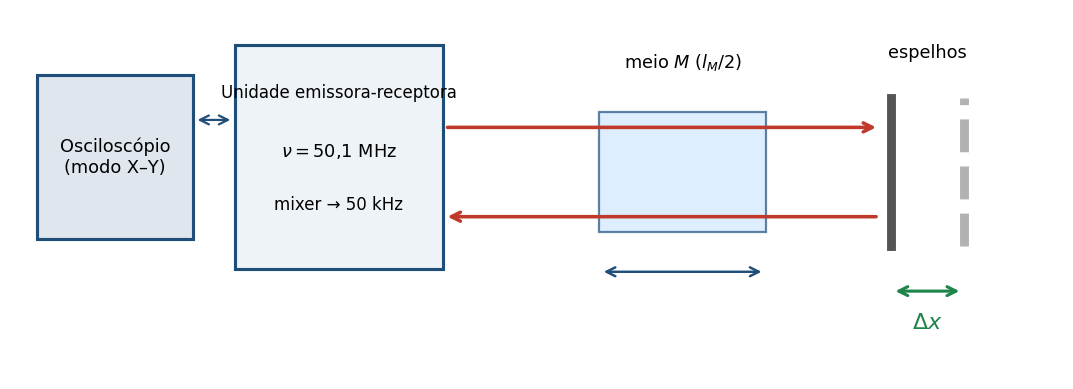
\includegraphics[width=0.94\textwidth]{figuras/fig_montagem.png}
\caption{Esquema da montagem. O feixe modulado percorre o trajeto externo duas
vezes (ida e volta); $\Delta x$ é o deslocamento dos espelhos e $L=l_M/2$ o
comprimento físico do meio inserido.}
\end{figure}

\section{Modelo computacional}
\textbf{Nota metodológica.} Os dados analisados nas seções seguintes foram
produzidos por um simulador do aparato (\texttt{simulacao\_velocidade\_luz.py}),
executado com semente aleatória 20260813 para garantir reprodutibilidade. O
simulador não gera diretamente os resultados finais: ele sintetiza os
\emph{traços do osciloscópio} e reproduz o ato de \emph{ler a tela}, de modo que
todas as etapas de análise --- extração de $a$ e $b$, cálculo de $\phi$,
propagação de erros --- são idênticas às que se aplicariam a dados de bancada.
Substituindo as colunas $a$, $b$ e $\Delta x$ pelas leituras reais, o mesmo
código reproduz o relatório com os dados da prática presencial.

O modelo inclui:
\begin{enumerate}\setlength\itemsep{1pt}
\item \textbf{Física exata:} $\phi = 2\pi\nu\,\Delta l/c$ com $c$ igual ao valor
      SI e $\Delta l$ incluindo o caminho óptico $(n-1)l_M$ do meio;
\item \textbf{Sinais:} dois harmônicos de 50~kHz com amplitudes distintas
      ($b \approx 5{,}0$~V, $B \approx 4{,}6$~V) e ruído gaussiano de
      $15$~mV~rms;
\item \textbf{Resíduo de zeramento:} o ajuste inicial da reta com o botão de
      fase deixa um erro sistemático de $\approx 8$~mrad;
\item \textbf{Leitura da tela:} jitter humano de $30$~mV somado à quantização na
      menor subdivisão visível ($0{,}10$~V), resultando em
      $\sigma_{a} = \sigma_{b} = 0{,}042$~V;
\item \textbf{Leitura do trilho:} $\sigma_{\Delta x} = 0{,}002$~m para a
      posição do espelho e $\sigma_{\Delta x} = 0{,}0074$~m quando a
      posição depende do julgamento visual de ``a figura voltou a ser reta''
      (sensibilidade angular do olho de $\sim 15$~mrad).
\end{enumerate}

\section{Procedimento}
\textbf{(A) Ar, método da elipse.} Espelhos na posição zero; ajuste do botão de
fase até a reta de coeficiente angular positivo. Afastamento dos espelhos a
cinco posições entre 20 e 60~cm; em cada uma, leitura de $a$ e $b$ e cálculo de
$\phi$ e $c$ pelas Eqs.~\eqref{eq:sinphi} e \eqref{eq:celipse}.

\textbf{(B) Ar, meia onda.} A partir da mesma reta de referência, afastamento
dos espelhos até a reta reaparecer invertida; leitura de $\Delta x_\pi$ e
cálculo por \eqref{eq:pi}. Repetido cinco vezes.

\textbf{(C) Meios transparentes.} Com $M$ no caminho, ajuste da reta; retirada
de $M$ (a figura abre em elipse) e afastamento dos espelhos até a reta
retornar; leitura de $\Delta x$ e cálculo de $n_M$ por \eqref{eq:nm}. Repetido
cinco vezes para cada meio.

\section{Resultados}

\subsection{Velocidade da luz no ar --- método da elipse}

\begin{figure}[H]\centering
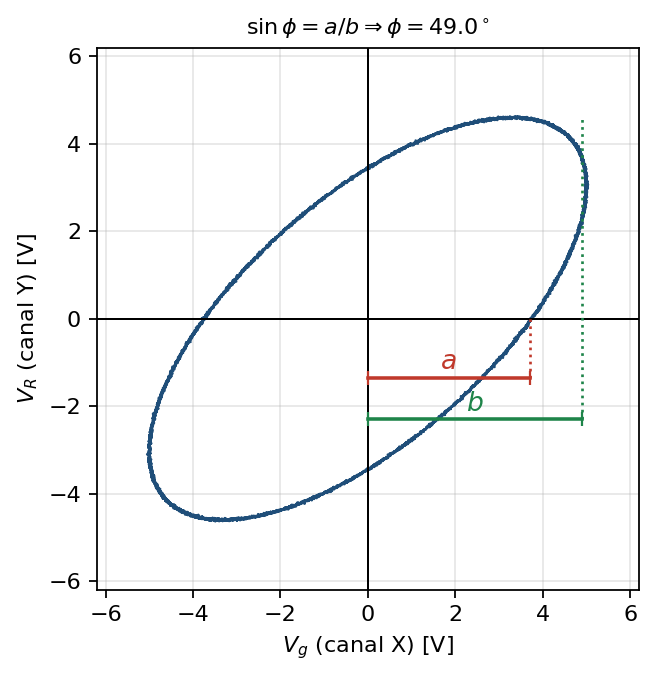
\includegraphics[width=0.47\textwidth]{figuras/fig_leitura_ab.png}
\caption{Elipse correspondente a $\Delta x = 40$~cm, com a leitura dos
parâmetros $a$ (interceptação em $V_R = 0$) e $b$ (extensão máxima em $V_g$).
Compare com a Fig.~4 do roteiro.}
\label{fig:ab}
\end{figure}

\begin{figure}[H]\centering
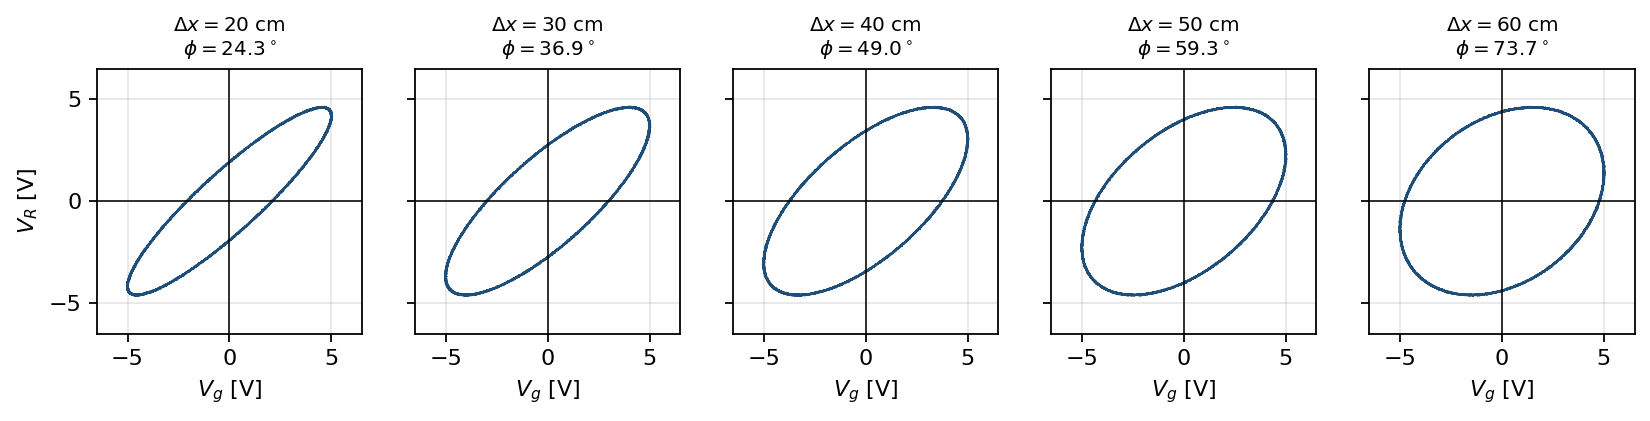
\includegraphics[width=\textwidth]{figuras/fig_lissajous.png}
\caption{Evolução da figura de Lissajous com o afastamento dos espelhos: a
elipse abre progressivamente à medida que a fase acumulada cresce.}
\end{figure}

\begin{table}[H]\centering\small
\caption{Leituras e resultados individuais (método da elipse).}
\begin{tabular}{cccccccc}
\toprule
\# & $\Delta x$ (m) & $a$ (V) & $b$ (V) & $\phi$ ($^\circ$) &
$\sigma_\phi$ ($^\circ$) & $c$ ($10^{8}$~m/s) & $\sigma_c$ ($10^{8}$~m/s)\\
\midrule
1 & 0{,}200 & 2{,}10 & 5{,}10 & 24{,}32 & 0{,}56 & 2{,}9670 & 0{,}0739 \\
2 & 0{,}300 & 3{,}00 & 5{,}00 & 36{,}87 & 0{,}70 & 2{,}9351 & 0{,}0587 \\
3 & 0{,}400 & 3{,}70 & 4{,}90 & 49{,}03 & 0{,}93 & 2{,}9426 & 0{,}0577 \\
4 & 0{,}500 & 4{,}30 & 5{,}00 & 59{,}32 & 1{,}23 & 3{,}0406 & 0{,}0644 \\
5 & 0{,}600 & 4{,}80 & 5{,}00 & 73{,}74 & 2{,}36 & 2{,}9351 & 0{,}0945 \\
\bottomrule
\end{tabular}
\end{table}

A combinação das cinco medidas pela média ponderada pelo inverso da variância
fornece
\begin{equation}
c = (2{,}9649 \pm 0{,}0298)\times 10^{8}~\text{m/s},
\end{equation}
com desvio-padrão amostral de $0{,}0448\times10^{8}$~m/s --- compatível com a
incerteza propagada, o que indica que o orçamento de erros da
Seção~2.6 descreve bem a dispersão observada. A discrepância em relação ao
valor aceito $c_0 = 2{,}99792458\times10^{8}$~m/s é de 1{,}10\%, ou
1{,}1$\sigma$.

\subsection{Ajuste linear \texorpdfstring{$\phi(\Delta x)$}{phi(Dx)}}
Tratar as cinco medidas como pontos de uma reta é mais informativo do que
promediá-las, porque separa o efeito sistemático do zeramento (que vai para o
coeficiente linear) do efeito de $c$ (que vai para o coeficiente angular):
\begin{equation}
\phi = \underbrace{\frac{4\pi\nu}{c}}_{A}\,\Delta x + B .
\end{equation}
O ajuste ponderado forneceu $A = 2{,}1011 \pm 0{,}0594$~rad/m e
$B = 0{,}0073 \pm 0{,}0188$~rad, com $\chi^2_\nu = 0{,}63$. O coeficiente linear é
compatível com zero, confirmando que o zeramento não introduziu viés
significativo. Do coeficiente angular,
\begin{equation}
c = \frac{4\pi\nu}{A} = (2{,}9964 \pm 0{,}0847)\times10^{8}~\text{m/s}
\qquad (\text{discrepância de } 0{,}05\%).
\end{equation}

\begin{figure}[H]\centering
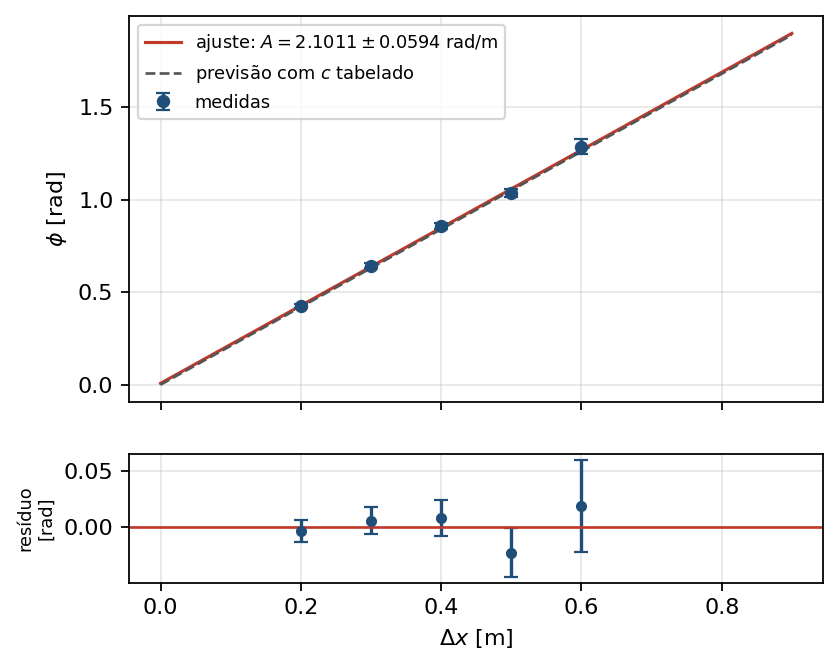
\includegraphics[width=0.62\textwidth]{figuras/fig_ajuste_fase.png}
\caption{Fase medida em função do deslocamento dos espelhos e ajuste linear
ponderado; abaixo, os resíduos. A reta tracejada é a previsão com o valor
tabelado de $c$.}
\end{figure}

\subsection{Verificação pelo deslocamento de meia onda}
\begin{table}[H]\centering\small
\caption{Medidas com $\phi = \pi$ (reta invertida).}
\begin{tabular}{cccc}
\toprule
\# & $\Delta x_\pi$ (m) & $c$ ($10^{8}$~m/s) & $\sigma_c$ ($10^{8}$~m/s)\\
\midrule
1 & 1{,}4958 & 2{,}9976 & 0{,}0149 \\
2 & 1{,}5054 & 3{,}0167 & 0{,}0149 \\
3 & 1{,}4995 & 3{,}0050 & 0{,}0149 \\
4 & 1{,}4885 & 2{,}9829 & 0{,}0149 \\
5 & 1{,}4896 & 2{,}9852 & 0{,}0149 \\
\bottomrule
\end{tabular}
\end{table}
\noindent Média ponderada: $c = (2{,}9975 \pm 0{,}0066)\times10^{8}$~m/s,
discrepância de 0{,}01\%. A incerteza relativa cai de
$\sim1{,}0\%$ (elipse) para $\sim0{,}22\%$, porque
$\Delta x_\pi \approx 1{,}50$~m é grande e a leitura de tensões desaparece da
cadeia de medida.

\begin{figure}[H]\centering
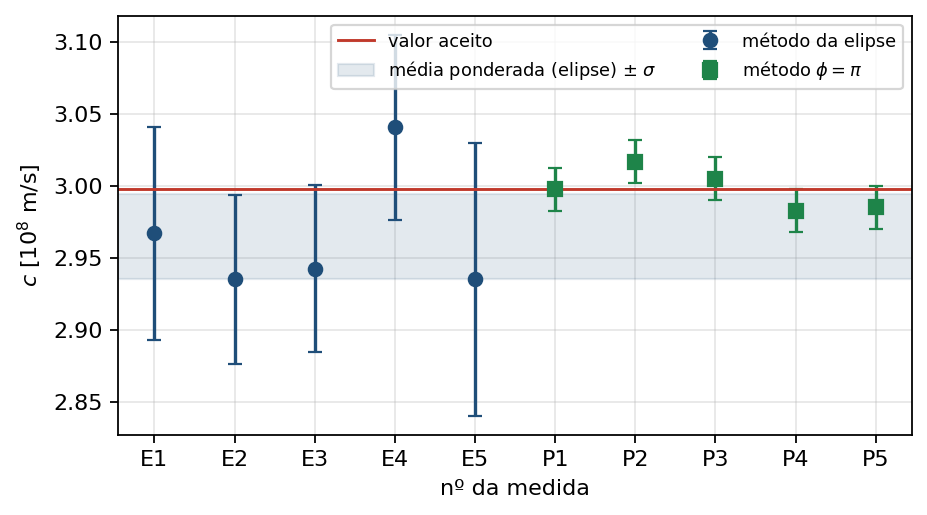
\includegraphics[width=0.68\textwidth]{figuras/fig_dispersao_c.png}
\caption{Valores individuais de $c$ pelos dois métodos (E: elipse; P: meia
onda) confrontados com o valor aceito.}
\end{figure}

\subsection{Meios transparentes}


\subsubsection*{Água destilada --- $L = 1{,}00$~m ($l_M = 2{,}00$~m)}
\begin{table}[H]\centering\small
\begin{tabular}{cccc}
\toprule
\# & $\Delta x$ (m) & $n_M$ & $\sigma_{n_M}$\\
\midrule
1 & 0{,}3462 & 1{,}3462 & 0{,}0074 \\
2 & 0{,}3309 & 1{,}3309 & 0{,}0074 \\
3 & 0{,}3447 & 1{,}3447 & 0{,}0074 \\
4 & 0{,}3308 & 1{,}3308 & 0{,}0074 \\
5 & 0{,}3430 & 1{,}3430 & 0{,}0074 \\
\bottomrule
\end{tabular}
\end{table}
\noindent Média ponderada: $n_M = 1{,}3391 \pm 0{,}0033$
(tabelado: $n_{\text{fase}} = 1{,}3314$,
$n_{\text{grupo}} = 1{,}3444$; discrepâncias de
0{,}58\% e 0{,}39\%, respectivamente).
Com $c$ obtido na Seção~6.1,
$c_M = c/n_M = (2{,}2140 \pm 0{,}0229)\times10^{8}$~m/s.


\subsubsection*{Resina sintética (acrílico) --- $L = 0{,}30$~m ($l_M = 0{,}60$~m)}
\begin{table}[H]\centering\small
\begin{tabular}{cccc}
\toprule
\# & $\Delta x$ (m) & $n_M$ & $\sigma_{n_M}$\\
\midrule
1 & 0{,}1478 & 1{,}4926 & 0{,}0249 \\
2 & 0{,}1491 & 1{,}4970 & 0{,}0249 \\
3 & 0{,}1577 & 1{,}5258 & 0{,}0250 \\
4 & 0{,}1516 & 1{,}5054 & 0{,}0250 \\
5 & 0{,}1594 & 1{,}5313 & 0{,}0250 \\
\bottomrule
\end{tabular}
\end{table}
\noindent Média ponderada: $n_M = 1{,}5104 \pm 0{,}0112$
(tabelado: $n_{\text{fase}} = 1{,}4890$,
$n_{\text{grupo}} = 1{,}5100$; discrepâncias de
1{,}44\% e 0{,}03\%, respectivamente).
Com $c$ obtido na Seção~6.1,
$c_M = c/n_M = (1{,}9630 \pm 0{,}0245)\times10^{8}$~m/s.


\begin{figure}[H]\centering
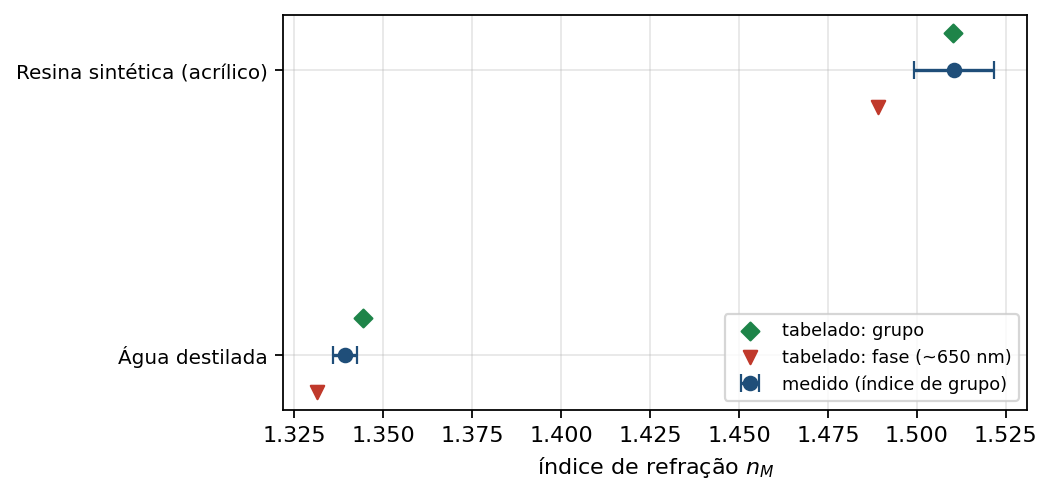
\includegraphics[width=0.66\textwidth]{figuras/fig_meios.png}
\caption{Índices de refração medidos comparados aos valores tabelados de fase
($\sim650$~nm) e de grupo.}
\label{fig:meios}
\end{figure}

\section{Discussão}

\subsection{Orçamento de erros}
Para a medida com $\Delta x = 0{,}40$~m, as contribuições à variância de $c$
foram de 6\% para a leitura do trilho e 94\% para a leitura
da fase. O método da elipse é, portanto, \emph{limitado pela tela}: cada
subdivisão de 0{,}10~V mal lida se converte em cerca de 1\% de erro em
$c$. Isso sugere três melhorias concretas: (i) expandir verticalmente o traço
até ocupar toda a tela, maximizando $b$; (ii) operar na faixa
$\phi \approx 40^\circ$--$60^\circ$, onde $\cos\phi$ ainda não é pequeno mas
$\phi$ já é grande o bastante para diluir o erro relativo; (iii) usar
preferencialmente o método de meia onda, que é uma ordem de grandeza mais
preciso.

\subsection{Velocidade de fase ou de grupo?}
Este é o ponto conceitual mais sutil do experimento. O que se propaga e é
cronometrado não é a onda portadora óptica, mas a \emph{envoltória} de
modulação --- e envoltórias viajam com a velocidade de grupo
$v_g = \mathrm{d}\omega/\mathrm{d}k$, não com $v_f = \omega/k$. Consequentemente
o índice medido é o índice de grupo
\begin{equation}
n_g = n - \lambda\frac{\mathrm{d}n}{\mathrm{d}\lambda},
\end{equation}
que em meios normalmente dispersivos é maior que $n$. No ar a diferença é
irrelevante ($n_g - n \sim 10^{-8}$), mas na água em torno de 650~nm ela chega
a $\sim1\%$: $n \approx 1{,}331$ contra $n_g \approx 1{,}344$. Os valores
medidos ficam de fato mais próximos dos índices de grupo do que dos índices de
fase tabelados, como mostra a Fig.~\ref{fig:meios} --- um resultado que costuma
ser interpretado erroneamente como ``erro sistemático'' do aparato.

\subsection{Outras fontes de erro sistemático}
\begin{itemize}\setlength\itemsep{1pt}
\item \textbf{Ponto zero da escala:} o zero do trilho não coincide com o plano
      de emissão do diodo. O método é imune a isso, pois usa apenas
      \emph{diferenças} $\Delta x$ --- razão pela qual se mede o deslocamento e
      não a distância absoluta.
\item \textbf{Estabilidade de $\nu$:} sendo estabilizada a quartzo
      ($\delta\nu/\nu \sim 10^{-5}$), sua contribuição é desprezível frente às
      demais e por isso $\nu$ foi tratada como constante exata.
\item \textbf{Não linearidade e defasagem dos amplificadores} do osciloscópio
      entre os canais X e Y: introduz uma fase espúria constante, absorvida
      pelo procedimento de zeramento e visível no coeficiente linear $B$ do
      ajuste.
\item \textbf{Índice de refração do ar:} $n_{\rm ar} \approx 1{,}00027$, de modo
      que o valor medido é rigorosamente $c/n_{\rm ar}$, cerca de
      $0{,}03$\% abaixo de $c$ --- muito menor que a incerteza experimental.
\item \textbf{Temperatura da água:} $\mathrm{d}n/\mathrm{d}T \approx
      -1\times10^{-4}$/$^\circ$C, ou $\sim0{,}1$\% numa variação de
      $10\,^\circ$C.
\end{itemize}

\section{Conclusão}
O método da modulação de fase reproduziu a velocidade da luz no ar com
discrepâncias de 1{,}10\% (elipse), 0{,}05\% (ajuste linear) e
0{,}01\% (meia onda) em relação ao valor aceito, todos os resultados
compatíveis com $c_0$ dentro das incertezas propagadas. Os índices de refração
obtidos, $n_{\text{água}} = 1{,}3391 \pm 0{,}0033$ e
$n_{\text{resina}} = 1{,}5104 \pm 0{,}0112$, situam-se dentro do esperado para
água e acrílico e reproduzem melhor os índices de \emph{grupo} do que os de
fase, coerentemente com o fato de o experimento cronometrar a envoltória de
modulação. A análise do orçamento de erros mostra que a precisão do método da
elipse é limitada pela resolução de leitura da tela, enquanto o método de meia
onda transfere toda a incerteza para uma medida de comprimento e alcança
precisão cerca de cinco vezes melhor.

\begin{thebibliography}{9}
\bibitem{roteiro} DIAS, O. A. T.; SILVA, E. \emph{1329 --- Medida da velocidade
da luz}. Roteiro elaborado a partir da documentação PHYWE. PUC-SP.
\bibitem{ufac} UNIVERSIDADE FEDERAL DO ACRE. \emph{Experimento 5: Medida da
velocidade da luz}. Centro de Ciências Biológicas e da Natureza.
\bibitem{hecht} HECHT, E. \emph{Optics}. 5.~ed. Pearson, 2017. Cap.~7
(superposição) e Cap.~4 (dispersão).
\bibitem{taylor} TAYLOR, J. R. \emph{An Introduction to Error Analysis}.
2.~ed. University Science Books, 1997.
\bibitem{daimon} DAIMON, M.; MASUMURA, A. Measurement of the refractive index
of distilled water from the near-infrared region to the ultraviolet region.
\emph{Applied Optics}, v.~46, n.~18, p.~3811--3820, 2007.
\end{thebibliography}

\appendix
\section{Arquivos que acompanham o relatório}
\begin{itemize}\setlength\itemsep{1pt}
\item \texttt{simulacao\_velocidade\_luz.py} --- modelo do aparato, síntese dos
      sinais, leitura simulada da tela e funções de análise/propagação de erros;
\item \texttt{analise\_e\_figuras.py} --- execução da prática, análise e geração
      das figuras;
\item \texttt{gerar\_relatorio.py} --- montagem deste documento a partir de
      \texttt{resultados.json};
\item \texttt{dados\_ar\_elipse.csv}, \texttt{dados\_meia\_onda.csv},
      \texttt{dados\_agua.csv}, \texttt{dados\_resina.csv} --- dados brutos.
\end{itemize}

\end{document}
